\chapter{Diffusion Models for RTI Fields}

\section{Introduction to score-based diffusion}

\subsection{From individual simulations to a probability distribution}

The objective of a generative surrogate is different from that of a deterministic
regression model. A deterministic model associates a single output with a given
input, whereas a generative model aims to describe the variability of all
admissible outputs. This distinction is essential for Rayleigh--Taylor
instability (RTI) simulations: small differences in the initial perturbations or
in the physical parameters may lead to significantly different interface
geometries and turbulent structures. Consequently, one reference field cannot
represent the full range of possible realizations.

Let $\mathbf{x}_0\in\mathbb{R}^{d}$ denote a discretized RTI density field, or
equivalently a vector containing the coefficients of one of the reduced
representations introduced in Chapter~2. The DNS dataset

\begin{equation}
    \mathcal{D}=\left\{\mathbf{x}_0^{(i)}\right\}_{i=1}^{N}
\end{equation}

is regarded as a finite collection of samples drawn from an unknown data
distribution $p_{\mathrm{data}}(\mathbf{x}_0)$. The central objective of this
report is therefore not to reconstruct one particular DNS realization, but to
learn the \emph{shape of the probability distribution} of the simulated RTI
fields. In other words, the model should assign high probability to physically
plausible density fields and low probability to configurations that are not
representative of the reference simulations.

The learned model, denoted by $p_{\theta}(\mathbf{x}_0)$, should approximate the
unknown distribution according to

\begin{equation}
    p_{\theta}(\mathbf{x}_0)\approx
    p_{\mathrm{data}}(\mathbf{x}_0).
\end{equation}

Once trained, it must be possible to draw new samples
$\widetilde{\mathbf{x}}_0\sim p_{\theta}$ that are not copies of the training
fields, while preserving their relevant statistical and physical properties.
For RTI, these properties include the morphology of bubbles and spikes, the
location and thickness of the mixing layer, the distribution of density values,
and the organization of structures across spatial scales. Thus, the quality of
the surrogate cannot be assessed from the visual fidelity of a single generated
field alone; it must also be evaluated by comparing ensembles of generated and
reference simulations.

Directly estimating $p_{\mathrm{data}}$ is difficult because each field belongs
to a high-dimensional space and the available number of DNS realizations is
limited. Diffusion models address this problem indirectly. Rather than imposing
a simple parametric form on the data distribution, they progressively transform
it into a tractable Gaussian distribution and learn how to reverse this
transformation.

\subsection{One-dimensional illustrative example}

Before considering RTI fields, it is useful to look at the same mechanism in
one dimension, where the whole probability distribution can be plotted. The
notebook \emph{1D-Simplest-Diffusion-Models} uses a toy dataset sampled from a
mixture of two Gaussian distributions,

\begin{equation}
    p_{\mathrm{data}}(x_0)
    =
    \sum_{k=1}^{2}
    \pi_k\,
    \mathcal{N}(x_0;\mu_k,\sigma_k^2),
\end{equation}

with modes centered around $\mu_1=-4$ and $\mu_2=4$. This distribution is
simple enough to visualize, but it already contains the main difficulty faced
by a generative model: the data are not concentrated around a single average
state. The model must instead represent two separated regions of high
probability, as illustrated in Figure~\ref{fig:diffusion_1d_dataset}.

\begin{figure}[H]
    \centering
    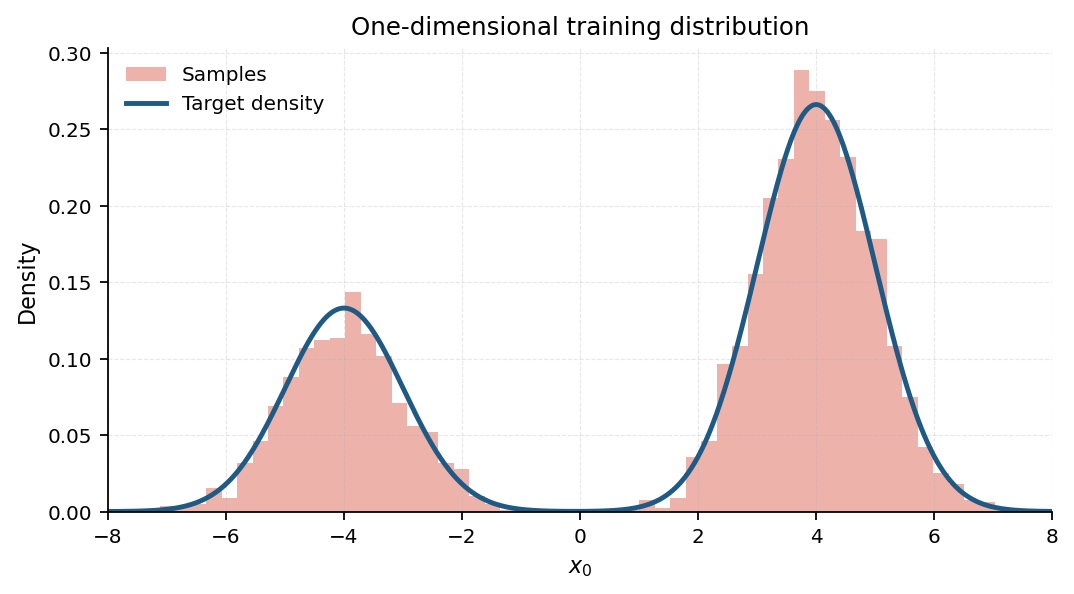
\includegraphics[width=0.70\textwidth]{figures/ch3/diffusion_1d_dataset.png}
    \caption{One-dimensional toy distribution used to illustrate diffusion.
    The histogram represents samples drawn from a bimodal Gaussian mixture,
    while the curve shows the corresponding probability density.}
    \label{fig:diffusion_1d_dataset}
\end{figure}

\subsection{Forward diffusion process}

The forward process is a fixed Markov chain that gradually corrupts a data
sample by adding Gaussian noise. Starting from
$\mathbf{x}_0\sim p_{\mathrm{data}}$, it is defined as

\begin{equation}
    q(\mathbf{x}_{1:T}\mid\mathbf{x}_0)
    =
    \prod_{t=1}^{T}
    q(\mathbf{x}_t\mid\mathbf{x}_{t-1}),
\end{equation}

with transition kernel

\begin{equation}
    q(\mathbf{x}_t\mid\mathbf{x}_{t-1})
    =
    \mathcal{N}\!\left(
        \mathbf{x}_t;
        \sqrt{1-\beta_t}\,\mathbf{x}_{t-1},
        \beta_t\mathbf{I}
    \right),
\end{equation}

where $\beta_t\in(0,1)$ controls the amount of noise introduced at step $t$.
Defining $\alpha_t=1-\beta_t$ and
$\overline{\alpha}_t=\prod_{s=1}^{t}\alpha_s$, any noisy state can be sampled
directly from the original field:

\begin{equation}
    \mathbf{x}_t
    =
    \sqrt{\overline{\alpha}_t}\,\mathbf{x}_0
    +
    \sqrt{1-\overline{\alpha}_t}\,\boldsymbol{\epsilon},
    \qquad
    \boldsymbol{\epsilon}\sim\mathcal{N}(\mathbf{0},\mathbf{I}).
\end{equation}

The first term progressively suppresses the information contained in the RTI
field, while the second replaces it with Gaussian noise. For a sufficiently
long and appropriately chosen noise schedule,
$q(\mathbf{x}_T)$ approaches the standard normal distribution
$\mathcal{N}(\mathbf{0},\mathbf{I})$. This mechanism is illustrated in the
one-dimensional notebook by a bimodal distribution: its two modes progressively
merge until the samples become approximately Gaussian. The same principle
applies to RTI fields, although their probability distribution lies in a much
higher-dimensional space and cannot be represented by a simple histogram.

Figure~\ref{fig:diffusion_1d_forward} gives a static view of this forward
corruption process for the one-dimensional example. At $t=0$, the density is
the original bimodal distribution. As $t$ increases, the means of the two modes
are multiplied by $\sqrt{\overline{\alpha}_t}$ and the random Gaussian part
dominates. The two modes therefore collapse toward the origin and the final
distribution becomes close to the standard normal prior used to start
generation.

\begin{figure}[H]
    \centering
    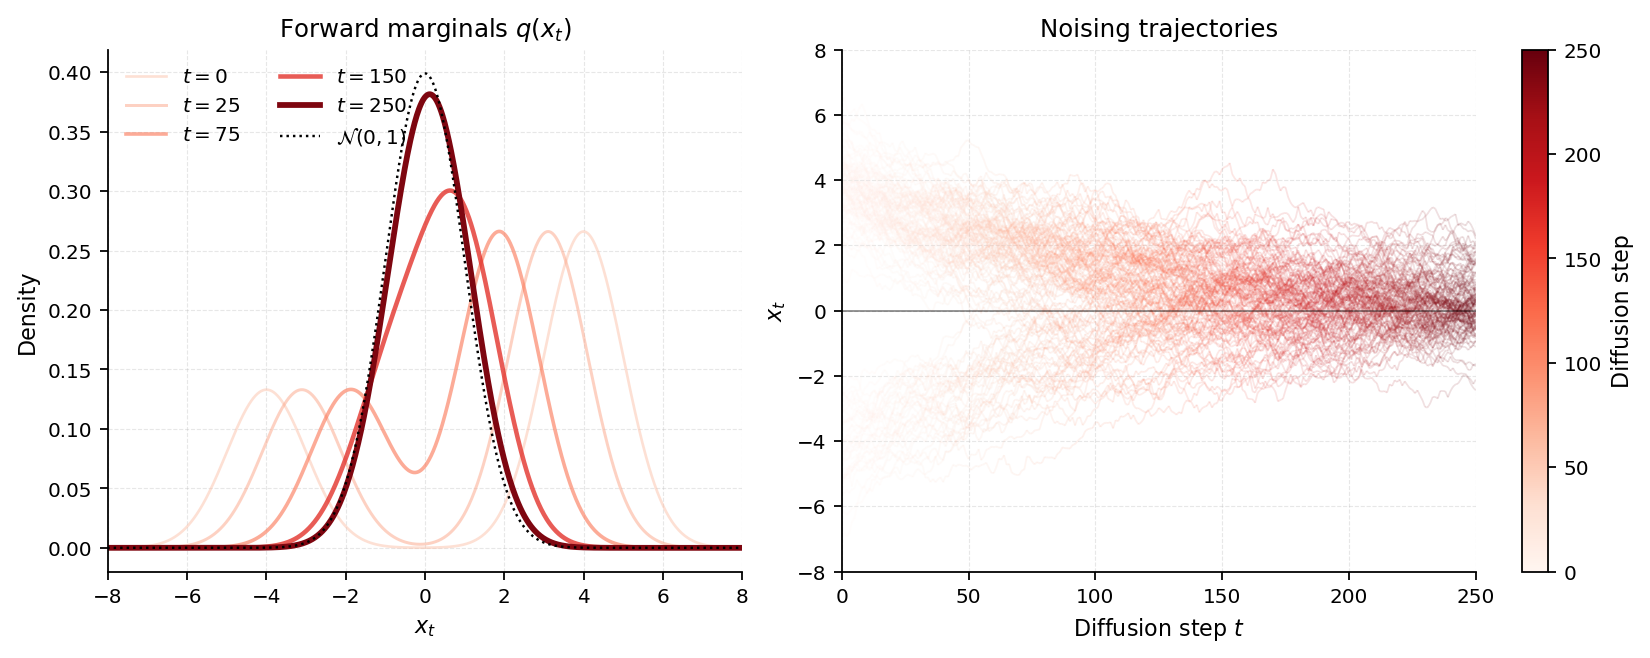
\includegraphics[width=0.95\textwidth]{figures/ch3/diffusion_1d_forward.png}
    \caption{Forward diffusion in one dimension. Left: evolution of the noisy
    marginal density $q(x_t)$ for several diffusion times. Right: trajectories
    of individual samples during the Markov noising process.}
    \label{fig:diffusion_1d_forward}
\end{figure}

\subsection{Learning the reverse process through the score}

Generation consists in reversing the corruption process. Starting from a
Gaussian sample $\mathbf{x}_T$, a neural network successively removes noise in
order to produce a sample $\mathbf{x}_0$. The reverse transitions are modeled
by

\begin{equation}
    p_{\theta}(\mathbf{x}_{0:T})
    =
    p(\mathbf{x}_T)
    \prod_{t=1}^{T}
    p_{\theta}(\mathbf{x}_{t-1}\mid\mathbf{x}_t).
\end{equation}

In the score-based formulation, the network learns the score of the noisy
distribution,

\begin{equation}
    \mathbf{s}_{\theta}(\mathbf{x}_t,t)
    \approx
    \nabla_{\mathbf{x}_t}\log p_t(\mathbf{x}_t),
\end{equation}

which points toward regions of higher probability density at each noise level.
In practice, an equivalent and commonly used parameterization trains a network
$\boldsymbol{\epsilon}_{\theta}$ to predict the Gaussian noise added to a clean
sample. A simplified training objective is

\begin{equation}
    \mathcal{L}_{\mathrm{simple}}(\theta)
    =
    \mathbb{E}_{\mathbf{x}_0,t,\boldsymbol{\epsilon}}
    \left[
        \left\|
        \boldsymbol{\epsilon}
        -
        \boldsymbol{\epsilon}_{\theta}(\mathbf{x}_t,t)
        \right\|_2^2
    \right].
\end{equation}

Because the model is trained over all noise levels, it learns a sequence of
local denoising directions rather than an explicit analytical expression for
the complex RTI distribution. Repeated application of these directions
transports samples from the Gaussian prior toward the regions occupied by the
DNS data. The resulting ensemble of generated fields provides an approximation
of the distribution sought in this work.

In the one-dimensional setting, the score can be represented as arrows along
the $x$ axis. These arrows point toward regions where the noisy density is
larger. Near the end of the forward process, the density is almost Gaussian and
the score mainly points back toward the origin. At lower noise levels, the
score separates the samples toward the two modes of the data distribution. The
reverse generative process can therefore be interpreted as a gradual
specialization: an initially structureless Gaussian sample is first brought
back to the high-probability region, then assigned to one of the modes.

\begin{figure}[H]
    \centering
    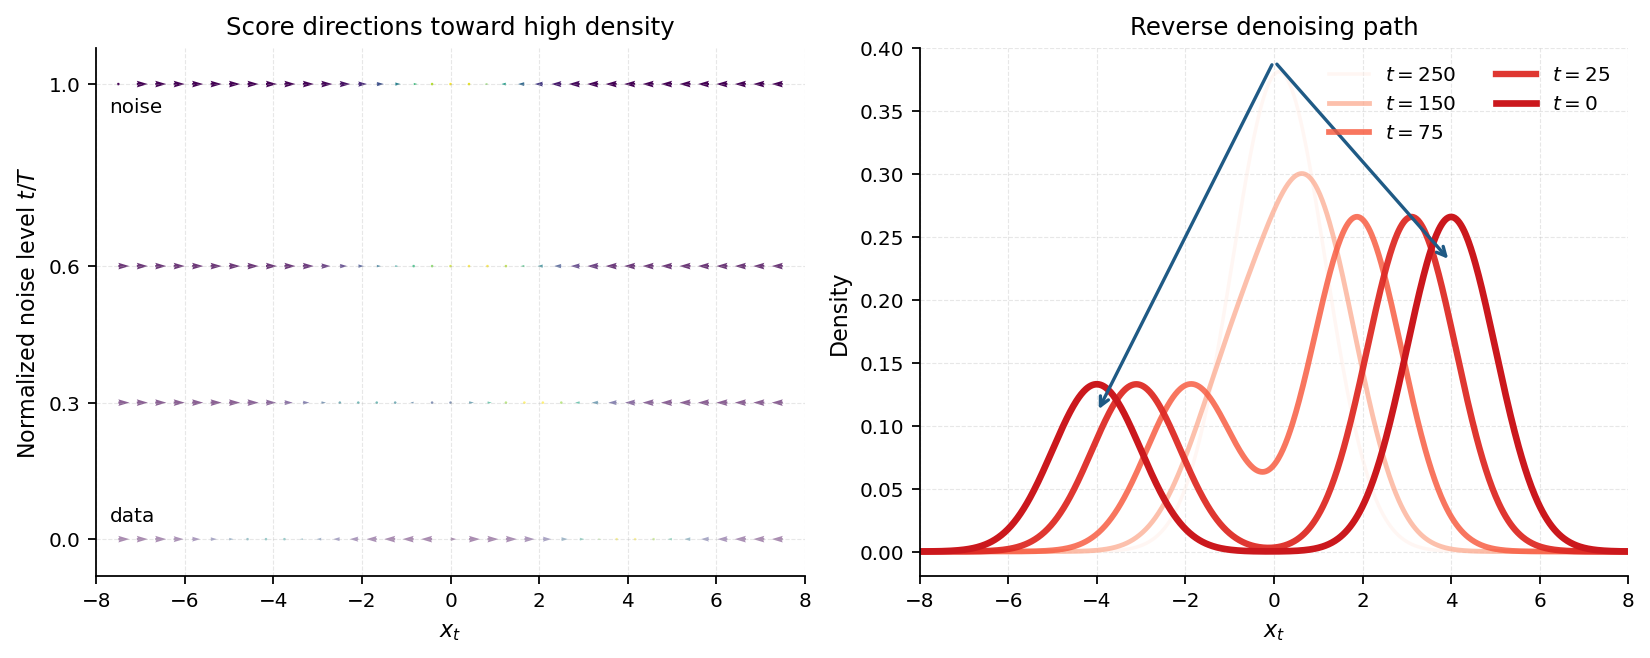
\includegraphics[width=0.95\textwidth]{figures/ch3/diffusion_1d_reverse_score.png}
    \caption{Score-based reverse process in the one-dimensional example. Left:
    score directions for several noise levels. Right: reverse denoising viewed
    as the transformation of the Gaussian prior back into the bimodal data
    distribution.}
    \label{fig:diffusion_1d_reverse_score}
\end{figure}


\section{Adaptation to RTI dataset}

\subsection{Data size}

Due to the high computational cost of Direct Numerical Simulations (DNS), the
number of available realizations is inherently limited. The dataset used in
this work consists of approximately 60 independent simulations of the
Rayleigh-Taylor instability. Each simulation produces thousands of temporal
snapshots during its execution; however, only a subset of these snapshots is
stored because of storage limitations. After preprocessing and filtering, the
final dataset contains fewer than 7000 images.

This dataset size is several orders of magnitude smaller than those typically
used to train diffusion models for natural image generation, where millions of
samples are commonly available. Such a limited amount of training data
increases the risk of overfitting and limits the ability of the model to learn
the underlying distribution of RTI density fields. Consequently, physically
consistent data augmentation techniques are employed during training to increase
the effective diversity of the dataset.

\subsection{Data augmentation} Since the dataset originates from numerical simulations rather than experimental measurements, the admissible data augmentations are constrained by the symmetries of the governing equations and by the numerical formulation of the DNS. The simulations are performed with a pseudo-spectral solver using periodic boundary conditions in the horizontal direction. Consequently, the flow is invariant under cyclic translations along the horizontal axis. Random horizontal shifts therefore preserve both the physical solution and its statistical properties. Likewise, the governing equations remain invariant under the reflection $x\rightarrow -x$, making horizontal flipping a physically consistent augmentation. On the other hand, the vertical direction is distinguished by the gravitational acceleration. Vertical translations modify the position of the mixing layer within the computational domain, while vertical reflections exchange the heavy and light fluids and reverse the direction of gravity. These operations no longer correspond to realizations of the original physical problem and are therefore excluded. For the same reason, arbitrary image rotations are not considered. During training, each sample is randomly augmented using horizontal cyclic translations and horizontal reflections only. These transformations increase the effective diversity of the training set while preserving the physical properties of the Rayleigh--Taylor instability.
The number of translation was fixed to 10 because the 1st model training was made with a 16x16 patch size.
\begin{figure}[H]
    \centering
    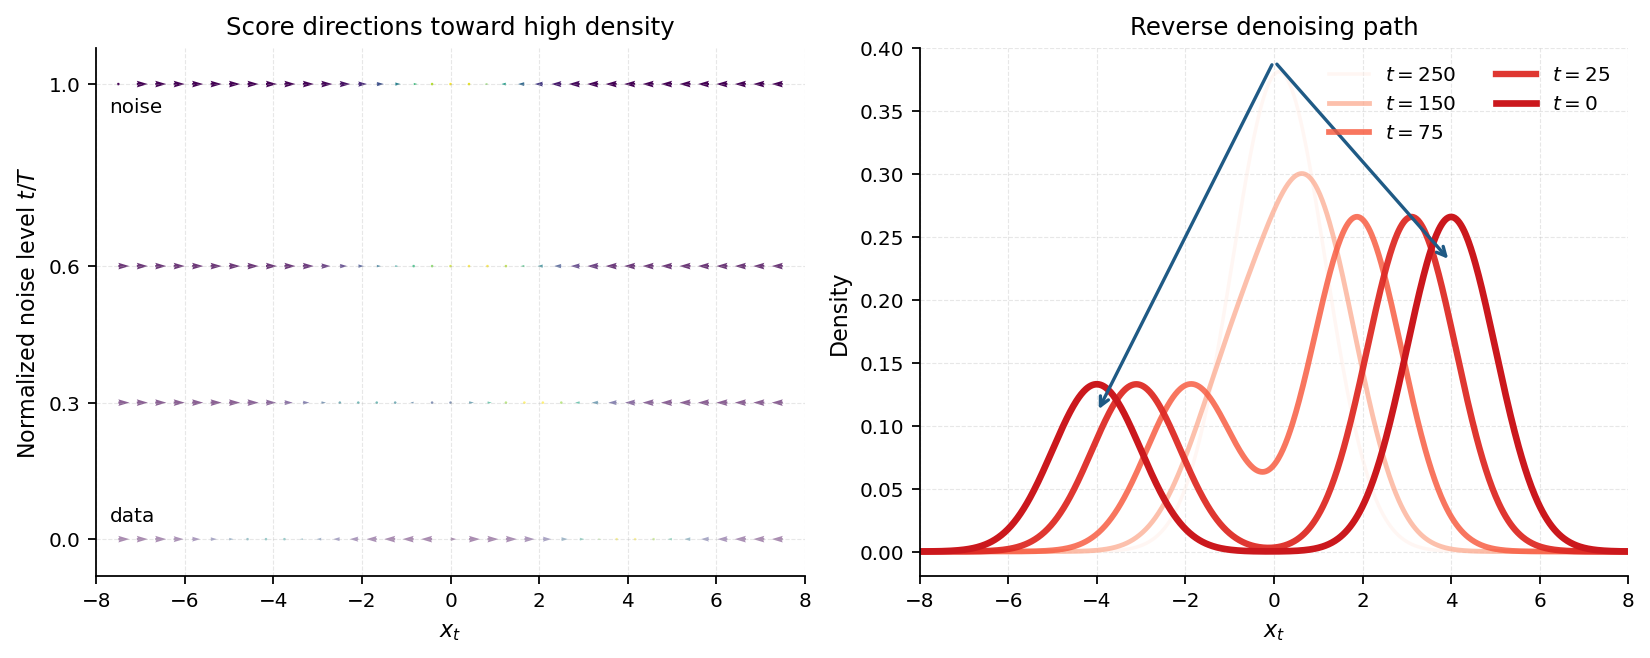
\includegraphics[width=0.95\textwidth]{figures/ch3/diffusion_1d_reverse_score.png}
    \caption{Score-based reverse process in the one-dimensional example. Left:
    score directions for several noise levels. Right: reverse denoising viewed
    as the transformation of the Gaussian prior back into the bimodal data
    distribution.}
    \label{fig:diffusion_1d_reverse_score}
\end{figure}


\subsection{Data ratio}
Unlike conventional image generation tasks, the geometry of the RTI dataset is
not chosen for computational convenience but is directly constrained by the
numerical formulation of the Direct Numerical Simulations (DNS).

The simulations are performed using a pseudo-spectral solver with periodic
boundary conditions in the horizontal direction. Consequently, every flow field
is periodically replicated outside the computational domain. If the largest
coherent structures become comparable to the domain width, they interact with
their own periodic images, introducing artificial correlations that modify the
physical evolution of the instability.

Let $L_x$ denote the horizontal size of the computational domain and
$L_b$ the characteristic diameter of the largest RTI bubbles. To avoid
significant finite-domain effects, the dominant structures must satisfy

\begin{equation}
    L_b \ll L_x
\end{equation}

In practice, a conservative criterion commonly adopted in pseudo-spectral DNS is

\begin{equation}
    L_b \lesssim \frac{L_x}{4}
\end{equation}

which ensures that the largest bubbles remain sufficiently separated from their
periodic replicas throughout the simulation.

The vertical direction obeys a different constraint. Since the mixing layer
continuously grows under the action of gravity, the computational domain must be
long enough to avoid interactions between the evolving interface and the
artificial numerical boundaries. For this reason, the domain is chosen much
taller than it is wide.

As a consequence, all simulations are generated on computational grids of
$128\times512$ points, corresponding to an aspect ratio of $1:4$. The horizontal
resolution is sufficient to accurately represent the largest admissible bubble
structures while preventing spurious periodic interactions, whereas the extended
vertical dimension allows the mixing layer to develop over long physical times
without being constrained by the finite size of the computational domain.

\begin{figure}[H]
    \centering
    
\includegraphics[width=0.65\textwidth]{figures/ch3/original.png}
    \caption{Original DNS simulations of the Rayleigh--Taylor instability. The aspect ratio of the computational domain is $1:4$, with a horizontal size of $128$ points and a vertical size of $512$ points.}
    \label{fig:original_dns}
\end{figure}

The original simulations are subsequently cropped from a $128\times512$ domain
to a square field of view in order to match the input geometry required by the
diffusion model. Let $y_b(t)$ and $y_s(t)$ denote respectively the vertical
positions of the lowest bubble tip and the highest spike tip. A cropped sample
is retained only if

\[
y_{\min}^{\mathrm{crop}} < y_b(t)
\quad\text{and}\quad
y_s(t) < y_{\max}^{\mathrm{crop}},
\]

ensuring that the complete mixing layer remains inside the observation window.
Consequently, every retained sample contains the full physical evolution of the
interface without introducing artificial truncation of large-scale coherent
structures.

\begin{figure}[H]
    \centering
    
\includegraphics[width=0.65\textwidth]{figures/ch3/zone_melange.png}
    \caption{Representation of $y_b(t)$ and $y_s(t)$ for every $x$ to ensure that the mixing zone (yellow) is fully contained within the cropped field of view.}
    \label{fig:zone_melange}
\end{figure}

\section{Model architecture}

\section{Training pipeline}

\section{Baseline results}
